\documentclass[11pt,a4paper]{article}
\usepackage{fontspec}
\usepackage[ngerman]{babel}
\usepackage{amsmath,amssymb}
\usepackage{booktabs,tabularx,array}
\usepackage{graphicx}
\usepackage{xcolor}
\usepackage{microtype}
\usepackage[font=small,labelfont=bf]{caption}
\usepackage{siunitx}
\sisetup{locale=DE,group-minimum-digits=4}
\usepackage[margin=2.5cm]{geometry}
\usepackage{enumitem}
\usepackage{tikz,pgfplots}
\pgfplotsset{compat=1.18}
\usetikzlibrary{positioning,arrows.meta,fit,calc,backgrounds}
\usepackage[hidelinks]{hyperref}

\graphicspath{{../../reports/figures/}}
\setlength{\parskip}{0.45em}
\setlength{\parindent}{0pt}

\definecolor{frozen}{HTML}{E6F1FB}
\definecolor{frozenline}{HTML}{185FA5}
\definecolor{train}{HTML}{EEEDFE}
\definecolor{trainline}{HTML}{534AB7}
\definecolor{fixed}{HTML}{F1EFE8}
\definecolor{fixedline}{HTML}{5F5E5A}
\definecolor{lossc}{HTML}{FAECE7}
\definecolor{lossline}{HTML}{993C1D}

\newcommand{\merke}[1]{%
  \par\smallskip\noindent\fcolorbox{trainline}{train}{\parbox{\dimexpr\linewidth-2\fboxsep-2\fboxrule}{\small\textbf{Kernaussage.} #1}}\par\smallskip}

\title{\textbf{Wie das Automix-Modell funktioniert}\\[0.3em]
\large Schritt-für-Schritt-Erklärung als Grundlage für das Paper}
\author{Projekt \emph{Automatic Mixing}, Deep Learning SS26}
\date{Stand: 22.~September 2026}

\begin{document}
\maketitle

\begin{abstract}
\noindent Wir stellen ein kleines neuronales Netz vor, das Orchesteraufnahmen
automatisch zu einem Stereomix zusammenstellt. Eingabe sind die einzelnen
Mikrofonspuren einer Aufnahme -- das Hauptsystem und die Stützmikrofone an
den Instrumenten. Für jede Spur sagt das Modell zwei Mischpult-Einstellungen
vorher: einen Pegel (Gain) und eine Position im Stereopanorama (Pan). Ein
eingefrorenes, vortrainiertes Audionetz (VGGish) beschreibt den Klang jeder
Spur; ein trainierbares mehrschichtiges Perzeptron mit nur \num{132100}
Parametern trifft daraus die Entscheidungen. Die Einstellungen werden über
ein differenzierbares Pan-Gesetz zu einem Stereosignal gemischt, sodass das
Modell allein aus fertigen Mischungen lernt, ohne je die „richtigen“
Reglerstellungen zu sehen. Auf zurückgehaltenen synthetischen Stücken mit
bekannter Aufstellung platziert das Modell die Instrumente mit einem mittleren
Fehler von \SI{5.8}{\degree} (Rauschgrenze \SI{2.5}{\degree}, Mitte-Tipp
\SI{17.1}{\degree}).
\end{abstract}

\tableofcontents
\bigskip

%=====================================================================
\section{Die Aufgabe: Was heißt hier „automatisch mischen“?}

Bei einer Orchesteraufnahme hängen viele Mikrofone gleichzeitig im Saal:
\begin{itemize}[nosep]
  \item \textbf{Hauptsystem:} wenige Mikrofone über dem Dirigenten, die das
    ganze Orchester als Klangbild einfangen, z.\,B. ein Decca-Tree aus drei
    Mikrofonen (links, Mitte, rechts) und oft zusätzlich ein Raum-Paar.
  \item \textbf{Stützmikrofone (Spots):} Mikrofone nah an einzelnen
    Instrumenten oder Gruppen, etwa an den ersten Violinen oder der Harfe.
\end{itemize}
Der Tonmeister mischt diese Spuren zu einem Stereosignal. Dazu stellt er für
jede Spur mindestens ein, \emph{wie laut} sie in den Mix eingeht (Gain), und
\emph{wo} sie im Stereobild erscheint (Pan). Genau diese beiden Entscheidungen
soll unser Modell übernehmen.

\paragraph{Formal.} Gegeben sind $N$ Mono-Spuren $s_1(t),\dots,s_N(t)$ eines
Stücks. Gesucht ist für jede Spur ein Gain $g_i \ge 0$ und ein Panoramawinkel
$\theta_i \in [0,\pi/2]$ (in Grad: \SIrange{0}{90}{\degree}), sodass der
daraus gemischte Stereomix
\begin{equation}
  \hat y_L(t) = \sum_{i=1}^{N} g_i \cos(\theta_i)\, s_i(t), \qquad
  \hat y_R(t) = \sum_{i=1}^{N} g_i \sin(\theta_i)\, s_i(t)
  \label{eq:mix}
\end{equation}
möglichst gut klingt -- im Training heißt das: möglichst nah an einem
Referenzmix $y = (y_L, y_R)$ liegt.

\paragraph{Bewusste Vereinfachung.} Das Modell wählt \emph{eine} feste
Einstellung pro Spur für das ganze Stück. Es gibt keine Pegelautomation,
keinen Equalizer, keinen Hall und keine Laufzeitkorrektur. Das macht das
Modell klein, die Ausgabe direkt interpretierbar (zwei Zahlen pro Spur, wie
an einem Mischpult) und die ganze Kette differenzierbar. Dass die Vereinfachung
nicht aus der Luft gegriffen ist, zeigen die echten Mischungen des
Spheres-Datensatzes: Sie lassen sich \emph{exakt} als Summe nach
Gleichung~\eqref{eq:mix} darstellen (Bestimmtheitsmaß $R^2 = 1{,}000$,
Abschnitt~\ref{sec:daten}).

\begin{table}[h]
\centering\small
\begin{tabular}{@{}ll@{}}
\toprule
Symbol & Bedeutung \\
\midrule
$N$ & Anzahl der Spuren eines Stücks (variabel, hier 4--37) \\
$s_i(t)$ & Audiosignal der Spur $i$ (mono) \\
$e_i \in \mathbb{R}^{128}$ & Klang-Embedding der Spur $i$ (VGGish) \\
$c \in \mathbb{R}^{128}$ & Kontextvektor: mittleres Embedding aller Spuren \\
$g_i \ge 0$ & Gain (linear), in dB: $20\log_{10} g_i$ \\
$\theta_i \in [0,\pi/2]$ & Panoramawinkel: $0$ = ganz links, $\pi/4$ = Mitte, $\pi/2$ = ganz rechts \\
$m_i \in \{0,1\}$ & Maske: 1 = echte Spur, 0 = Auffüll-Spur im Batch \\
$\hat y,\; y$ & vorhergesagter Stereomix, Referenzmix \\
\bottomrule
\end{tabular}
\caption{Notation.}
\end{table}

%=====================================================================
\section{Überblick: Der Weg durch das Modell}

Abbildung~\ref{fig:pipeline} zeigt die gesamte Kette. Sie besteht aus vier
Bausteinen, von denen \emph{nur einer} trainiert wird:

\begin{enumerate}[nosep]
  \item \textbf{VGGish-Encoder} (eingefroren): beschreibt den Klang jeder Spur
    als Vektor $e_i$.
  \item \textbf{Kontext} (keine Parameter): Mittelwert aller $e_i$ -- „was
    spielt in diesem Stück sonst noch mit?“
  \item \textbf{MLP} (trainierbar): entscheidet aus $e_i$ und Kontext $c$
    über Gain $g_i$ und Pan $\theta_i$.
  \item \textbf{Mixer} (keine Parameter): wendet die Einstellungen nach
    Gleichung~\eqref{eq:mix} an und summiert zum Stereomix.
\end{enumerate}
Im Training vergleicht eine Verlustfunktion den Mix mit einer Referenz; der
Fehler fließt als Gradient durch den Mixer zurück in das MLP.

\begin{figure}[h]
\centering
\begin{tikzpicture}[
  node distance=5mm and 9mm,
  box/.style={draw, rounded corners=2pt, align=center, font=\small, minimum height=9mm, inner sep=4pt},
  fro/.style={box, fill=frozen, draw=frozenline},
  tra/.style={box, fill=train, draw=trainline, line width=0.9pt},
  fix/.style={box, fill=fixed, draw=fixedline},
  los/.style={box, fill=lossc, draw=lossline},
  arr/.style={-{Stealth[length=2.2mm]}, thick},
  lab/.style={font=\scriptsize, midway, fill=white, inner sep=1.5pt}]
  \node[fix, minimum width=30mm] (in) {Spuren $s_1,\dots,s_N$\\ \scriptsize (mono, \SI{44.1}{kHz})};
  \node[fro, below=of in, minimum width=30mm] (vgg) {VGGish-Encoder\\ \scriptsize eingefroren, 72,1 Mio.\ Param.};
  \node[fix, below=of vgg, minimum width=30mm] (emb) {Embeddings $e_i\in\mathbb{R}^{128}$};
  \node[fix, right=of emb, minimum width=30mm] (ctx) {Kontext $c$\\ \scriptsize Mittelwert über Spuren};
  \node[tra, below=9mm of emb, xshift=20mm, minimum width=52mm] (mlp) {MLP (pro Spur, geteilte Gewichte)\\ \scriptsize trainierbar, \num{132100} Parameter};
  \node[fix, below=of mlp, minimum width=40mm] (gt) {Gain $g_i$ \quad Pan $\theta_i$};
  \node[fix, left=16mm of gt, minimum width=24mm] (anc) {Anker\\ \scriptsize feste $\theta$ fürs\\ \scriptsize Hauptsystem};
  \node[fix, below=of gt, minimum width=40mm] (mix) {Mixer: Pan-Gesetz\\ \scriptsize Gl.~\eqref{eq:mix}, summiert};
  \node[fix, below=of mix, minimum width=40mm] (out) {Stereomix $\hat y=(\hat y_L,\hat y_R)$};
  \node[los, right=12mm of out, minimum width=30mm] (loss) {Verlust\\ \scriptsize MR-STFT, 4 Ansichten};
  \node[fix, above=of loss, minimum width=30mm] (tgt) {Referenzmix $y$\\ \scriptsize (nur im Training)};

  \draw[arr] (in) -- (vgg);
  \draw[arr] (vgg) -- (emb);
  \draw[arr] (emb) -- (ctx);
  \draw[arr] (emb.south) -- ++(0,-4.5mm) -| ([xshift=-12mm]mlp.north);
  \draw[arr] (ctx.south) -- ++(0,-4.5mm) -| ([xshift=12mm]mlp.north);
  \draw[arr] (mlp) -- (gt);
  \draw[arr] (anc) -- node[above, font=\scriptsize]{ersetzt $\theta$} (gt);
  \draw[arr] (gt) -- (mix);
  \draw[arr] (in.west) -- ++(-30mm,0) |- (mix.west);
  \draw[arr] (mix) -- (out);
  \draw[arr] (out) -- (loss);
  \draw[arr] (tgt) -- (loss);
  \draw[arr, dashed, draw=lossline] (loss.east) -- ++(6mm,0) |- node[pos=0.25, right, font=\scriptsize, text=lossline, align=left]{Gradient\\(nur ins MLP)} (mlp.east);
\end{tikzpicture}
\caption{Die Pipeline. Blau: eingefroren. Violett: der einzige trainierte
Baustein. Grau: feste Rechenschritte ohne Parameter. Die Rohspuren gehen
zweimal ein: einmal zur Klangbeschreibung, einmal direkt in den Mixer.}
\label{fig:pipeline}
\end{figure}

\merke{Das Modell erzeugt keinen Klang, es erzeugt Reglerstellungen. Das
Audio selbst wird nur skaliert und im Panorama verteilt. Dadurch kann das
Modell keine Artefakte „erfinden“, und seine Entscheidungen sind so lesbar
wie ein Mischpult.}

%=====================================================================
\section{Schritt 1: Vom Audio zum Klangvektor -- der VGGish-Encoder}

Damit das Netz entscheiden kann, \emph{was} auf einer Spur zu hören ist, muss
das Audio in eine kompakte Beschreibung übersetzt werden. Dafür verwenden wir
VGGish \cite{hershey2017}, ein Faltungsnetz, das auf einer sehr großen Menge
von Videotonspuren darauf trainiert wurde, Geräusch- und Musikklassen zu
erkennen.

\paragraph{Ablauf für eine Spur.}
\begin{enumerate}[nosep]
  \item Die Spur wird von \SI{44.1}{kHz} auf \SI{16}{kHz} umgetastet
    (VGGish erwartet diese Rate).
  \item Sie wird in Abschnitte von \SI{0.96}{s} geschnitten; für jeden
    Abschnitt wird ein logarithmisches Mel-Spektrogramm berechnet, also eine
    Darstellung der Energie über Zeit und gehörangepassten Frequenzbändern.
  \item Das Faltungsnetz bildet jeden Abschnitt auf einen Vektor mit 128
    Zahlen ab.
  \item Die Vektoren aller Abschnitte werden gemittelt. Ergebnis: \emph{ein}
    Vektor $e_i \in \mathbb{R}^{128}$ pro Spur.
\end{enumerate}

\paragraph{Warum eingefroren?} VGGish hat rund 72,1 Millionen Parameter. Mit
unseren wenigen Trainingsdaten (Abschnitt~\ref{sec:daten}) ließen sich diese
nicht sinnvoll nachtrainieren -- das Netz würde die Trainingsstücke auswendig
lernen. Eingefroren liefert VGGish dagegen eine robuste, allgemeine
Klangbeschreibung, und trainiert wird nur der kleine Entscheidungsteil.

\paragraph{Was im Vektor steckt.} Vor allem die \emph{Klangfarbe}: Eine
Geigen-Spur und eine Posaunen-Spur landen an deutlich verschiedenen Stellen.
Zum Teil auch der \emph{Pegel}: Wird dieselbe Spur um \SI{24}{dB} leiser
gemacht, verschiebt sich der Vektor spürbar (Abstand 0,93 bei einer
Vektorlänge von etwa 2,5). Das ist wichtig, denn ohne Pegelinformation könnte
das Modell keinen passenden Gain wählen.

\paragraph{Was verloren geht.} Durch die Mittelung über die Zeit weiß das
Modell nicht, \emph{wann} ein Instrument spielt oder wie sich die Dynamik
entwickelt -- passend zur Entscheidung für statische Einstellungen, aber eine
klare Grenze (Abschnitt~\ref{sec:grenzen}).

%=====================================================================
\section{Schritt 2: Der Kontext -- was spielt sonst noch mit?}

Wie laut und wo eine Geige gemischt wird, hängt davon ab, was sonst im Stück
passiert: Im Streichquartett ist sie Hauptstimme, in der Sinfonie eine von
vielen. Deshalb bekommt jede Spur zusätzlich einen \emph{Kontextvektor}, den
Mittelwert über alle Spuren des Stücks:
\begin{equation}
  c = \frac{\sum_{i=1}^{N} m_i\, e_i}{\sum_{i=1}^{N} m_i}.
  \label{eq:ctx}
\end{equation}

\paragraph{Wozu die Maske $m_i$?} Im Training werden mehrere Stücke
gleichzeitig verarbeitet (ein \emph{Batch}). Weil Stücke unterschiedlich viele
Spuren haben, werden kürzere Listen mit stummen Platzhalterspuren aufgefüllt.
Die Maske sorgt dafür, dass diese Platzhalter weder in den Mittelwert noch
später in den Mix eingehen.

\paragraph{Zwei nützliche Eigenschaften.}
\begin{itemize}[nosep]
  \item \textbf{Beliebige Spurzahl:} Ein Mittelwert funktioniert für 4 wie für
    37 Spuren.
  \item \textbf{Reihenfolge egal:} Vertauscht man die Spuren, ändert sich $c$
    nicht, und jede Spur bekommt dieselbe Entscheidung. Das Modell ist
    \emph{permutationsäquivariant} -- die Dateireihenfolge spielt keine Rolle.
\end{itemize}

%=====================================================================
\section{Schritt 3: Die Entscheidung -- das MLP}

Das mehrschichtige Perzeptron (MLP) ist der einzige Teil, der lernt. Es
bekommt für jede Spur ihren eigenen Klangvektor und den Kontext, hintereinander
gehängt zu einem Vektor mit 256 Zahlen, und gibt zwei Zahlen aus.

\begin{table}[h]
\centering\small
\begin{tabular}{@{}llr@{}}
\toprule
Schicht & Form & Parameter \\
\midrule
Eingabe $[e_i; c]$ & 256 & -- \\
Linear + PReLU + Dropout 0,1 & $256 \to 256$ & \num{65793} \\
Linear + PReLU + Dropout 0,1 & $256 \to 256$ & \num{65793} \\
Linear & $256 \to 2$ & \num{514} \\
\midrule
\multicolumn{2}{@{}l}{Summe} & \num{132100} \\
\bottomrule
\end{tabular}
\caption{Architektur des MLP. PReLU ist eine Aktivierungsfunktion mit
lernbarer Steigung im negativen Bereich; Dropout schaltet im Training zufällig
10\,\% der Neuronen ab und beugt so dem Auswendiglernen vor.}
\end{table}

Die beiden Rohausgaben $z_1, z_2$ werden in gültige Reglerstellungen umgerechnet:
\begin{equation}
  g_i = \operatorname{softplus}(z_1) = \ln\!\left(1+e^{z_1}\right) \ge 0,
  \qquad
  \theta_i = \frac{\pi}{2}\,\sigma(z_2) = \frac{\pi}{2}\cdot\frac{1}{1+e^{-z_2}} \in \left[0,\tfrac{\pi}{2}\right].
\end{equation}
Softplus garantiert einen nicht-negativen Gain, die Sigmoid-Funktion $\sigma$
einen Winkel zwischen ganz links und ganz rechts. Zu Beginn des Trainings
liegen die Ausgaben nahe null, also $\theta \approx \pi/4$: Jede Spur startet
in der Mitte.

\paragraph{Geteilte Gewichte.} Für jede Spur wird \emph{dasselbe} MLP
verwendet. Das Modell lernt also keine Regel „Spur Nummer 3 nach links“,
sondern „eine Spur, die \emph{so} klingt, in einem Stück, das \emph{so} klingt,
gehört dorthin“. Nur deshalb funktioniert es auf Aufnahmen mit anderen
Spurnamen und anderer Spurzahl.

%=====================================================================
\section{Schritt 4: Anker -- feste Positionen für das Hauptsystem}

Bei den Mikrofonen des Hauptsystems ist die Stereoposition physikalisch
vorgegeben: Das linke Tree-Mikrofon gehört nach links, das rechte nach rechts.
Diese Spuren werden über ihren Dateinamen erkannt (z.\,B. \texttt{*\_L},
\texttt{*\_C}, \texttt{*\_R}, \texttt{*\_RoomL}) und bekommen einen festen
Winkel: \SI{0}{\degree}, \SI{45}{\degree} bzw.\ \SI{90}{\degree}. Der
vorhergesagte Winkel wird für sie verworfen; ihren \emph{Gain} wählt das Modell
aber weiterhin selbst.

Anker haben zwei Vorteile: Sie geben dem Stereobild eine eindeutige
Orientierung (Abschnitt~\ref{sec:loss}) und nehmen dem Modell Entscheidungen ab,
die ohnehin feststehen. Wichtig in der Anwendung: Beim Mischen eines neuen
Stücks muss dieselbe Ankerliste gelten wie im Training.

%=====================================================================
\section{Schritt 5: Der Mixer -- ein differenzierbares Pan-Gesetz}
\label{sec:mixer}

Der Mixer setzt Gleichung~\eqref{eq:mix} um. Der Anteil einer Spur im linken
und rechten Kanal ist $g\cos\theta$ bzw.\ $g\sin\theta$. Weil
$\cos^2\theta + \sin^2\theta = 1$ gilt, bleibt die abgestrahlte
\emph{Leistung} einer Spur an jeder Panoramaposition gleich
(\emph{Constant-Power-Panning}): Ein Instrument wird beim Verschieben nicht
lauter oder leiser. In der Mitte ($\theta=\SI{45}{\degree}$) erhält jeder Kanal
den Faktor $\cos\SI{45}{\degree} \approx 0{,}707$, also \SI{-3}{dB}
(Abbildung~\ref{fig:panlaw}).

\begin{figure}[h]
\centering
\begin{tikzpicture}
\begin{axis}[width=10cm, height=5.2cm, xmin=0, xmax=90, ymin=0, ymax=1.05,
  xlabel={Panoramawinkel $\theta$ in Grad}, ylabel={Faktor},
  xtick={0,22.5,45,67.5,90}, xticklabels={0 (L),22{,}5,45 (Mitte),67{,}5,90 (R)},
  ytick={0,0.25,0.5,0.707,1}, yticklabels={0,0{,}25,0{,}5,0{,}707,1},
  grid=major, grid style={gray!25}, legend pos=south west, legend style={font=\small, fill=white, fill opacity=0.9},
  every axis plot/.append style={thick, samples=91}]
  \addplot[domain=0:90, color=frozenline] {cos(x)};
  \addlegendentry{links: $\cos\theta$}
  \addplot[domain=0:90, color=lossline] {sin(x)};
  \addlegendentry{rechts: $\sin\theta$}
  \addplot[domain=0:90, color=gray, dashed] {cos(x)^2+sin(x)^2};
  \addlegendentry{Leistung $\cos^2\!+\sin^2$}
\end{axis}
\end{tikzpicture}
\caption{Das Constant-Power-Pan-Gesetz. Die Gesamtleistung einer Spur (grau
gestrichelt) ist unabhängig von ihrer Position.}
\label{fig:panlaw}
\end{figure}

\merke{Der Mixer ist die entscheidende Idee des Ansatzes. Weil er aus lauter
differenzierbaren Operationen besteht (Multiplikationen, Kosinus, Sinus,
Summen), lässt sich berechnen, wie sich der Fehler des fertigen Mixes ändert,
wenn man einen Regler ein wenig verstellt. Das Modell braucht deshalb
\emph{keine} Beispiele für „richtige“ Reglerstellungen -- es lernt allein
aus Paaren von Einzelspuren und fertigem Mix. Diese Idee eines
differenzierbaren Mischpults geht auf Steinmetz et~al.\ \cite{steinmetz2021}
zurück; unser Mischpult ist bewusst auf Gain und Pan reduziert.}

%=====================================================================
\section{Schritt 6: Wie gut ist der Mix? -- die Verlustfunktion}
\label{sec:loss}

Die Verlustfunktion misst, wie weit der vorhergesagte Mix $\hat y$ von der
Referenz $y$ entfernt ist. Ein direkter Vergleich der Wellenformen Sample für
Sample wäre ungeeignet: Er reagiert extrem empfindlich auf kleinste
Phasenunterschiede, die man nicht hört. Stattdessen vergleichen wir
\emph{Spektrogramme}, also die Energie über Zeit und Frequenz.

\paragraph{Ein Spektrogramm-Vergleich.} Für ein Signal wird mit der
Kurzzeit-Fouriertransformation (STFT, Hann-Fenster der Länge $n$, Schrittweite
$n/4$) das Betragsspektrogramm $|X|$ berechnet. Zwei Maße werden addiert:
\begin{align}
  \mathcal{L}_{\text{SC}} &= \frac{\big\| |Y| - |\hat Y| \big\|_F}{\big\| |Y| \big\|_F},\\
  \mathcal{L}_{\text{LM}} &= \frac{1}{K}\big\| \log(|Y|+\varepsilon) - \log(|\hat Y|+\varepsilon) \big\|_1 .
\end{align}
Die \emph{Spectral Convergence} $\mathcal{L}_{\text{SC}}$ misst die relative
Abweichung und wird von den lauten Anteilen dominiert. Der
\emph{Log-Magnitude}-Term $\mathcal{L}_{\text{LM}}$ vergleicht logarithmierte
Beträge; er gewichtet leise Anteile stärker und liegt näher an der
Lautheitswahrnehmung des Gehörs. $\|\cdot\|_F$ ist die Frobenius-Norm, $K$ die
Anzahl der Spektrogramm-Einträge, $\varepsilon = 10^{-8}$.

\paragraph{Mehrere Auflösungen.} Ein langes Fenster löst Frequenzen fein auf,
aber Zeit grob -- ein kurzes umgekehrt. Deshalb wird der Vergleich bei drei
Fenstergrößen $n \in \{512, 1024, 2048\}$ gerechnet und gemittelt
(\emph{Multi-Resolution-STFT-Verlust}, MR-STFT \cite{yamamoto2020,arik2019}):
\begin{equation}
  \mathcal{L}_{\text{MR}}(\hat x, x) = \frac{1}{3}\sum_{n\in\{512,1024,2048\}}
  \Big(\mathcal{L}_{\text{SC}}^{(n)} + \mathcal{L}_{\text{LM}}^{(n)}\Big).
\end{equation}

\paragraph{Vier Ansichten des Stereosignals.} Der Gesamtverlust vergleicht vier
aus dem Stereosignal abgeleitete Signale:
\begin{equation}
  \begin{aligned}
  \mathcal{L} = {}&
  \underbrace{\mathcal{L}_{\text{MR}}(\hat y_L+\hat y_R,\; y_L+y_R)}_{\text{Summe (Mitte)}}
  + \underbrace{\mathcal{L}_{\text{MR}}(\hat y_L-\hat y_R,\; y_L-y_R)}_{\text{Differenz (Breite)}}\\
  &+ \underbrace{\mathcal{L}_{\text{MR}}(\hat y_L,\; y_L)}_{\text{links}}
  + \underbrace{\mathcal{L}_{\text{MR}}(\hat y_R,\; y_R)}_{\text{rechts}}.
  \end{aligned}
  \label{eq:loss}
\end{equation}
Summe und Differenz stammen aus \cite{steinmetz2021}. Die beiden Kanalterme
haben wir ergänzt, und sie sind für Orchester entscheidend:

\paragraph{Das Spiegel-Problem.} Vertauscht man in einem Mix links und
rechts, bleibt die Summe $L+R$ gleich, und die Differenz $L-R$ wechselt nur
das Vorzeichen -- ihr Betragsspektrum ist identisch. Ein Verlust, der nur Summe
und Differenz vergleicht, kann einen Mix also nicht von seinem Spiegelbild
unterscheiden. Für Pop-Musik, wo die Seitenwahl oft beliebig ist, ist das
gewollt \cite{steinmetz2021}. Im Orchester gibt es dagegen eine feste
Sitzordnung. In unseren frühen Versuchen hat das Modell diese Blindheit
ausgenutzt und fast alles auf eine Seite gelegt (Pegelunterschied links zu
rechts bis \SI{+22.7}{dB}). Die Kanalterme in Gleichung~\eqref{eq:loss}
bestrafen Energie auf der falschen Seite und beheben dieses Kollabieren; die
Anker (Schritt~4) wirken zusätzlich strukturell in dieselbe Richtung.

%=====================================================================
\section{Schritt 7: Das Training}
\label{sec:daten}

\subsection{Daten}

\begin{table}[h]
\centering\small
\begin{tabularx}{\linewidth}{@{}lXl@{}}
\toprule
Datensatz & Beschreibung & Umfang \\
\midrule
Spheres & Echte Aufnahmen mit echtem Tonmeister-Mix (Hauptsystem L/C/R, Raum-Paar, Spots). Die Mischungen sind exakt statische Gain/Pan-Summen ($R^2=1{,}000$); je zwei Songs teilen dieselben Einstellungen. & 4 Songs, 2 Mischungen, \SI{5.7}{min} \\
SynthSOD & Synthetisch gerenderte Orchesterstücke, jedes Instrument einzeln pro Mikrofonposition (Close Mic ohne Übersprechen, Tree als Hauptsystem). & 576 Stücke, davon 64 genutzt \\
Synthmix & Unsere Neuberechnung der SynthSOD-Ziele: Spots nach einem festen Sitzplan im Panorama verteilt (plus $\pm\SI{5}{\degree}$ Zufall), Gains zufällig. Die wahren Werte werden pro Stück gespeichert. & 64 Stücke \\
\bottomrule
\end{tabularx}
\caption{Trainingsdaten. Die Synthmix-Ziele machen die Genauigkeit der
Positionen direkt messbar, weil die richtige Antwort bekannt ist.}
\end{table}

Der Sitzplan von Synthmix folgt der üblichen Orchesteraufstellung aus
Zuhörersicht (Violine~1 \SI{15}{\degree}, Violine~2 \SI{30}{\degree},
Viola \SI{55}{\degree}, Cello \SI{70}{\degree}, Kontrabass \SI{80}{\degree},
Holzbläser um die Mitte, Blech halbrechts). Die zurückgerechneten Einstellungen
der beiden echten Spheres-Tonmeister bestätigen ihn weitgehend: Violine~1 bei
\SIrange{9.5}{16}{\degree}, Viola bei \SIrange{57}{59}{\degree}, Horn bei
\SIrange{30}{31}{\degree}.

\subsection{Ablauf}
\begin{itemize}[nosep]
  \item \textbf{Aufteilung nach Stücken:} 10\,\% der Stücke (7 von 68) werden
    für die Validierung zurückgehalten -- ganze Stücke, nicht einzelne
    Ausschnitte, damit das Modell dort wirklich Unbekanntes sieht.
  \item \textbf{Ausschnitte:} Pro Epoche werden \num{1000} zufällige
    Ausschnitte von \SI{5}{s} Länge gezogen; zur Validierung dienen feste 200
    Ausschnitte.
  \item \textbf{Optimierung:} Adam \cite{kingma2015} mit Lernrate
    $3\cdot10^{-4}$, Batchgröße 16. Verbessert sich der Validierungsverlust
    20 Epochen lang nicht, wird die Lernrate halbiert.
  \item \textbf{Nur das MLP} wird optimiert; VGGish bleibt unverändert.
  \item \textbf{Rechenzeit:} Das Training lief auf einer Kaggle-GPU,
    etwa \SI{2.5}{min} pro Epoche.
\end{itemize}

\begin{figure}[h]
\centering
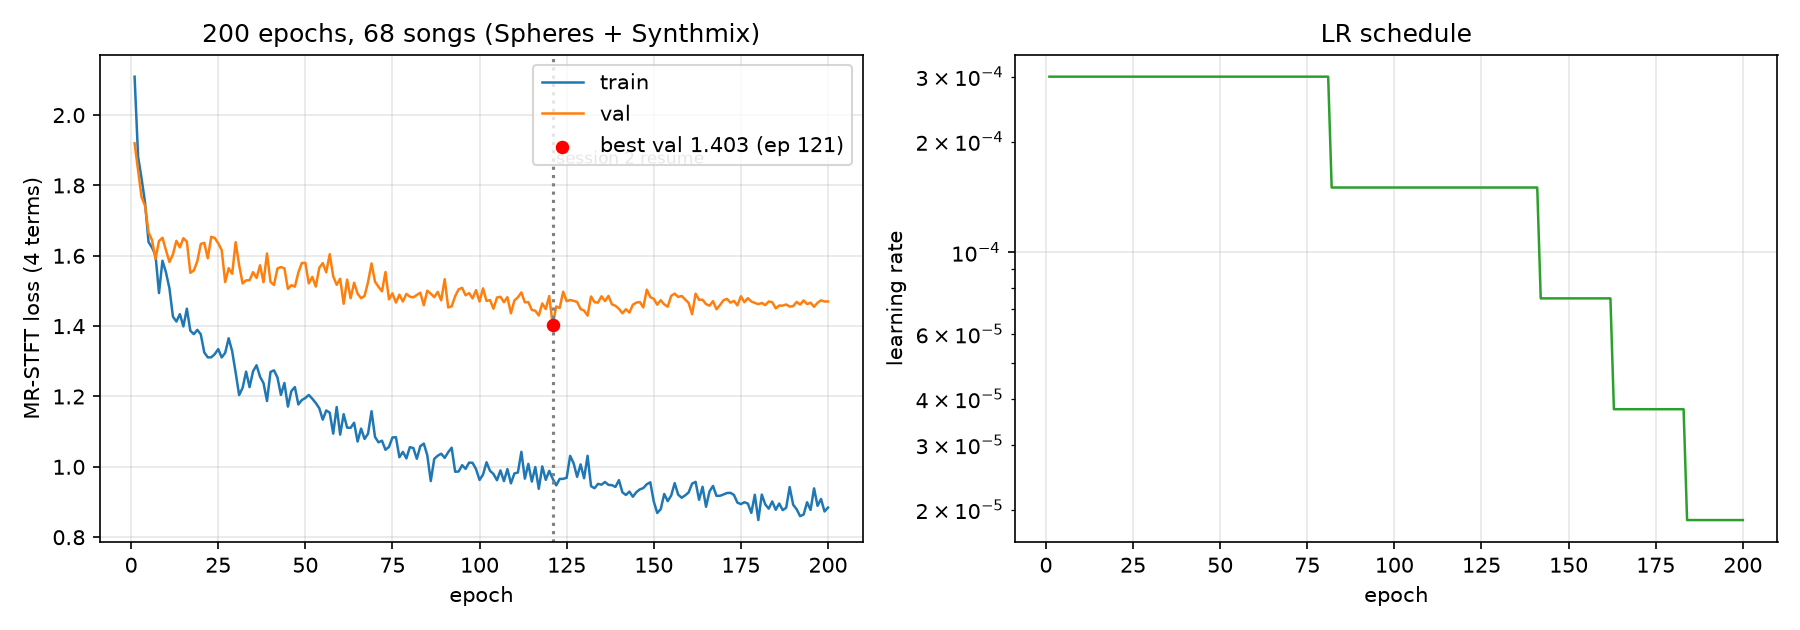
\includegraphics[width=\linewidth]{training_curves_200ep.png}
\caption{Verlustkurven des 200-Epochen-Laufs. Der beste Validierungsverlust
wird in Epoche 121 erreicht; danach sinkt nur noch der Trainingsverlust
(leichtes Overfitting).}
\end{figure}

\subsection{Experiment: Die echten Mischungen stärker gewichten}
\label{sec:spheresexp}
Bei gleichverteilter Auswahl stammen nur etwa 7\,\% der Ausschnitte aus
Spheres, dem einzigen Datensatz mit echten Tonmeister-Entscheidungen. In einem
zweiten Lauf bekam Spheres deshalb 40\,\% der Ausschnitte, erweitert um zwei
Datenaugmentierungen:
\begin{itemize}[nosep]
  \item \textbf{Pegelvariation:} Jede Spur wird beim Laden zufällig um bis zu
    $\pm\SI{6}{dB}$ lauter oder leiser gemacht, das Ziel bleibt gleich. Der
    richtige Gain verschiebt sich damit um den Gegenwert -- das Modell muss den
    Pegel aus dem Audio ablesen.
  \item \textbf{Spur-Dropout:} Zufällig weggelassene Spots werden mit ihrem
    exakten Anteil vom Ziel abgezogen. Aus zwei Mischungen entstehen so viele
    gültige Teilbesetzungen.
\end{itemize}
Alles andere -- Aufteilung, Modell, Verlustfunktion, Synthmix-Ziele -- blieb
gleich. \textbf{Kein einziges Maß wurde besser} (Tabelle~\ref{tab:spheresexp}).

\begin{table}[h]
\centering\small
\begin{tabular}{@{}lrr@{}}
\toprule
Maß & 200-Epochen-Lauf & Spheres-Gewichtung \\
\midrule
Pan-Fehler, unbekannte Stücke & \textbf{\SI{5.4}{\degree}} & \SI{6.6}{\degree} \\
Pan-Fehler, Spheres (im Training) & \textbf{\SI{7.9}{\degree}} & \SI{8.2}{\degree} \\
Gain-Fehler, Spheres (im Training) & \textbf{\SI{2.69}{dB}} & \SI{2.89}{dB} \\
Trainingsverlust am Ende & \textbf{0,97} & 1,63 \\
\bottomrule
\end{tabular}
\caption{Beide Läufe, jeweils mit dem Stand der letzten Epoche gemessen.}
\label{tab:spheresexp}
\end{table}

Aufschlussreich ist die Art des Scheiterns. Der Trainingsverlust blieb bei
1{,}63 stehen, obwohl die Lernrate schon stark reduziert war
(Abbildung~\ref{fig:curves2}), und die Tschaikowsky-Pegel blieben beim Fehler
eines konstanten Tipps -- \emph{obwohl} diese Stücke im Training waren, mit
sechsfachem Gewicht. Das Modell lernt die zwei echten Mischungen also nicht
auswendig, es kann sie überhaupt nicht nachbilden.

\merke{Der Engpass ist der Pegel, nicht die Datenmenge. Ein über die Zeit
gemitteltes VGGish-Embedding und ein Verlust, der nur Betragsspektren
vergleicht, geben dem MLP zu wenig Information über den Pegel einer Spur. Die
Pegelvariation hat die Aufgabe zusätzlich erschwert, ohne die nötige
Information zu liefern.}

\begin{figure}[h]
\centering
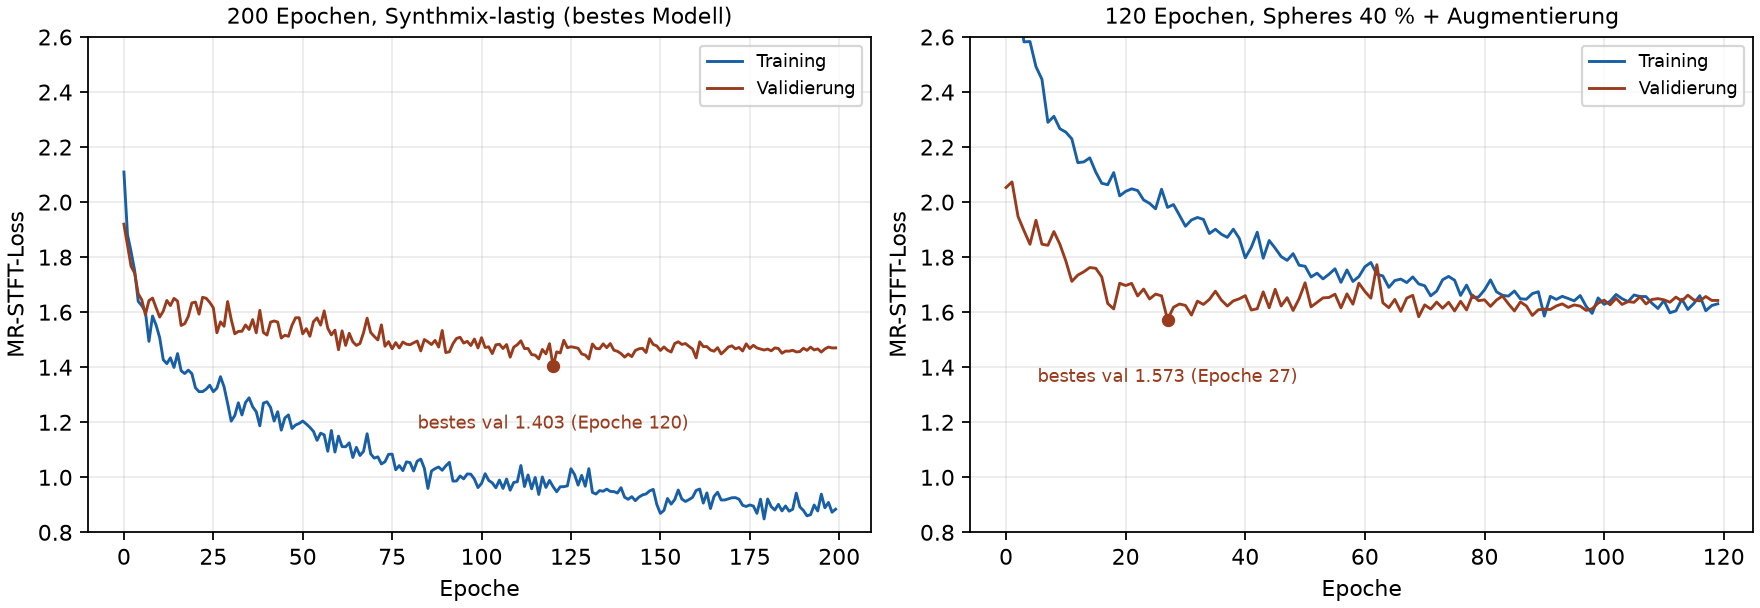
\includegraphics[width=\linewidth]{training_curves_comparison.png}
\caption{Links der 200-Epochen-Lauf (bestes Modell), rechts der Lauf mit
Spheres-Gewichtung. Rechts liegen Trainings- und Validierungskurve am Ende
übereinander: Das ist kein Overfitting, sondern Underfitting.}
\label{fig:curves2}
\end{figure}

%=====================================================================
\section{Schritt 8: Anwendung auf ein neues Stück}

Nach dem Training wird ein neues Stück so gemischt:
\begin{enumerate}[nosep]
  \item Alle Spuren werden geladen; Spuren des Hauptsystems erhalten ihre
    Anker-Winkel.
  \item VGGish beschreibt jede Spur über ihre \emph{gesamte} Länge
    (Mittelwert über alle \SI{0.96}{s}-Abschnitte des Stücks).
  \item Das MLP liefert einmal Gain und Pan pro Spur.
  \item Der Mixer wendet diese festen Einstellungen auf das ganze Stück an.
\end{enumerate}
Das Ergebnis ist ein vollständiger Stereomix und zugleich eine lesbare
Mischpult-Einstellung (Abbildung~\ref{fig:console}).

\begin{figure}[h]
\centering
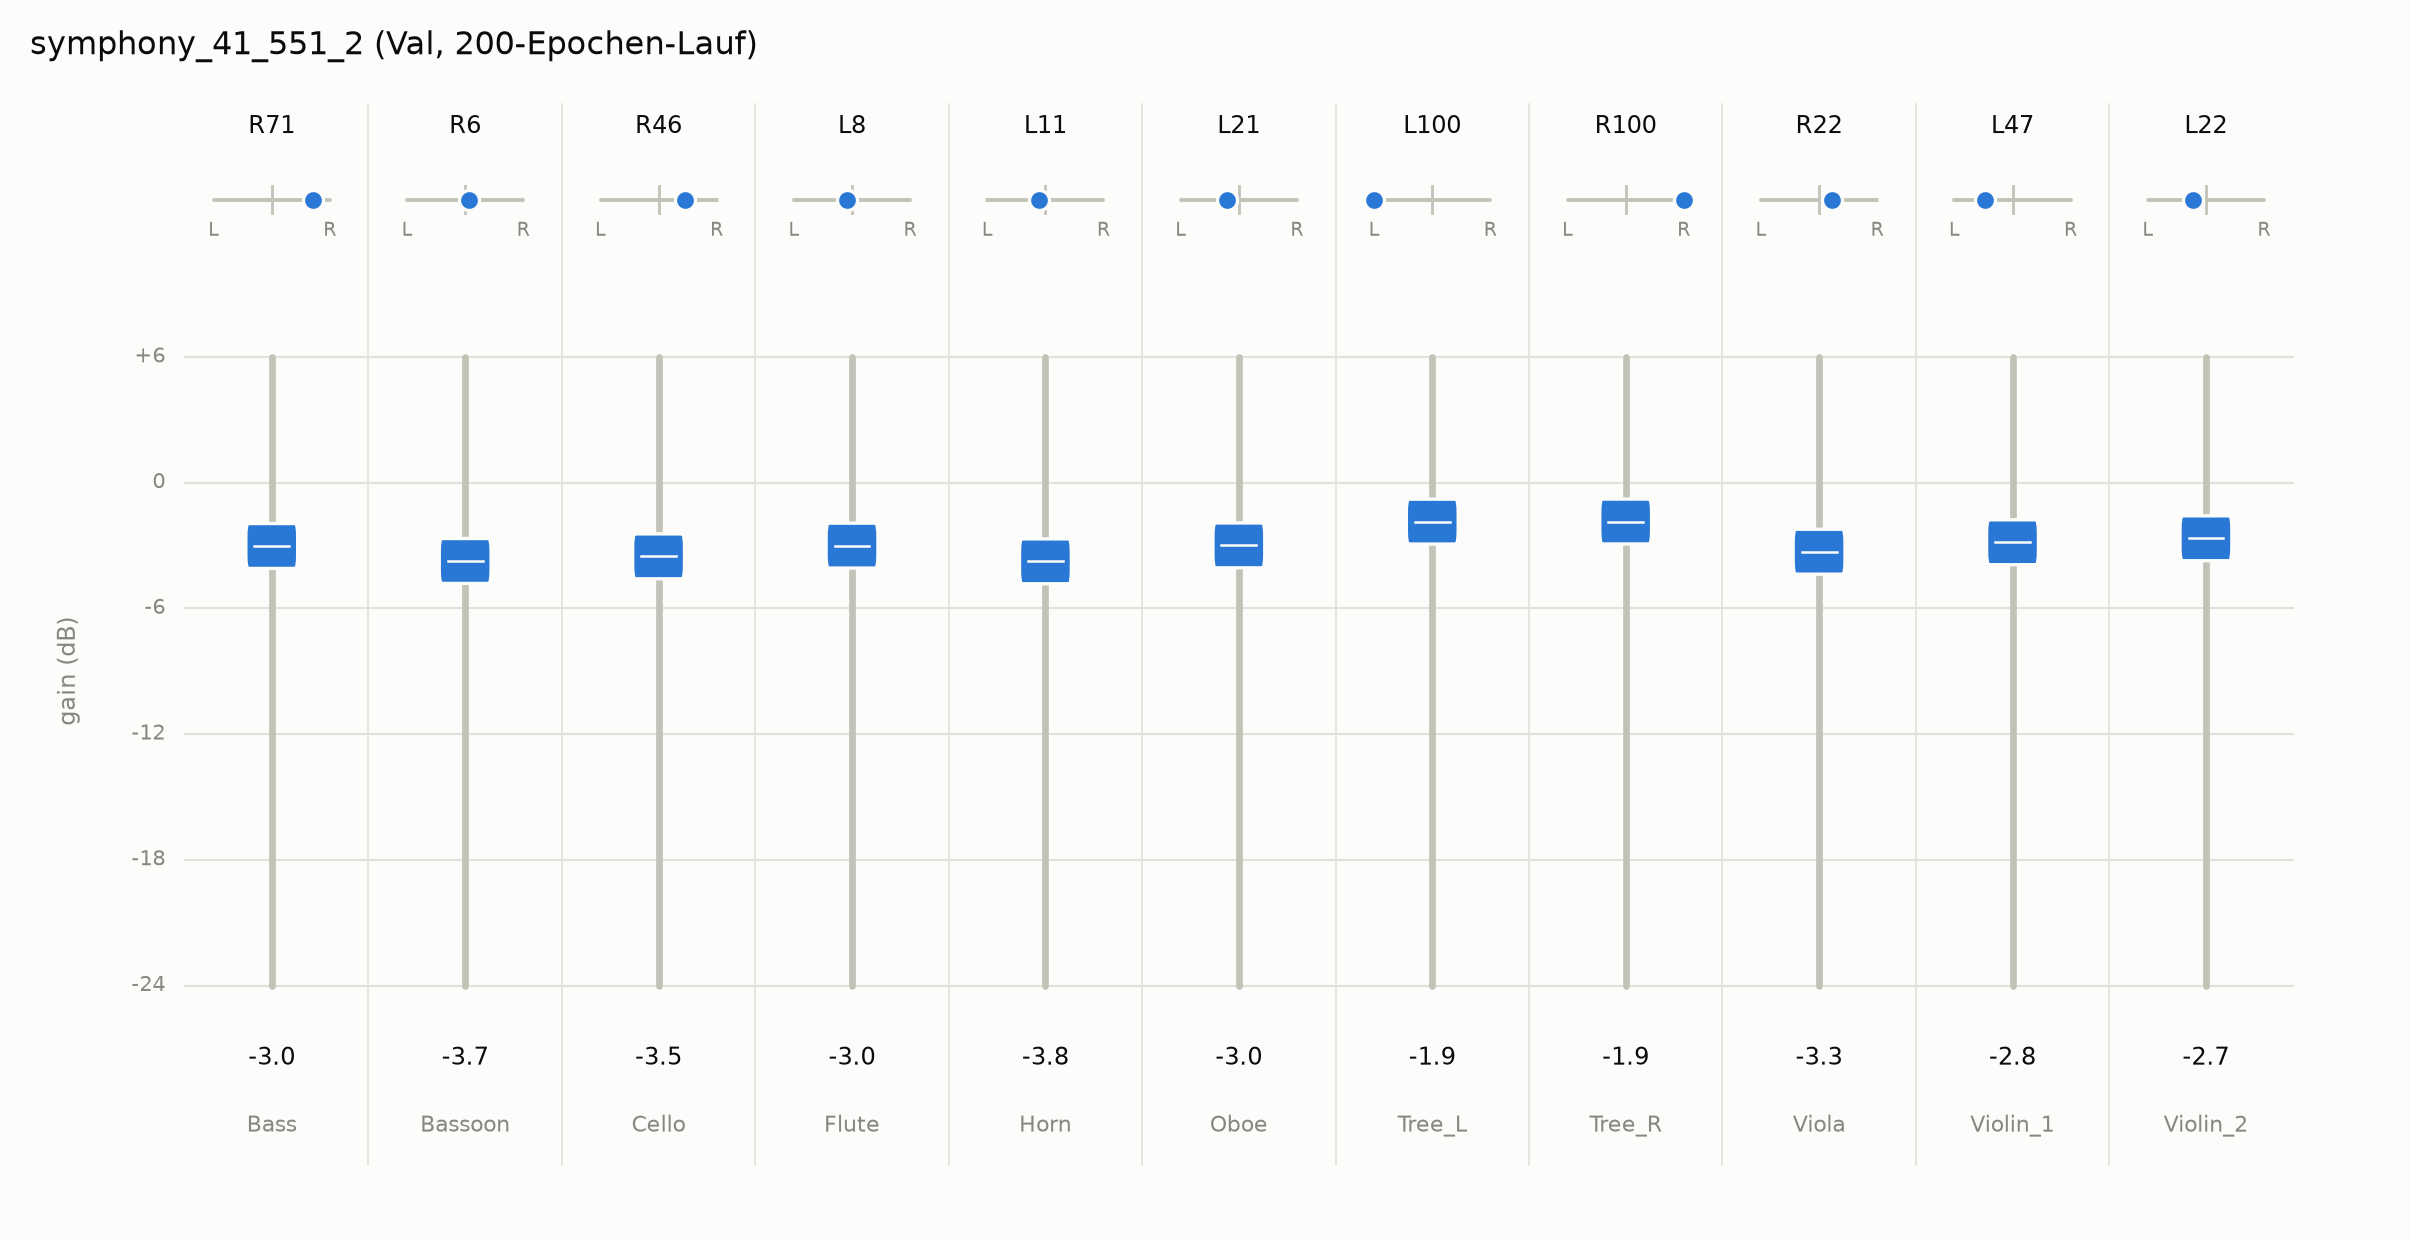
\includegraphics[width=\linewidth]{console_symphony.png}
\caption{Vom Modell gewählte Einstellungen für ein zurückgehaltenes Stück
(Sinfonie, 11 Spuren): oben die Panoramaposition, darunter der Fader. Die
Spuren Tree\_L und Tree\_R (Hauptsystem) sind Anker.}
\label{fig:console}
\end{figure}

%=====================================================================
\section{Was das Modell kann -- Ergebnisse im Überblick}

\paragraph{Positionen auf unbekannten Stücken (Synthmix-Validierung).}
Gemessen auf den 7 zurückgehaltenen Stücken mit bekannter Aufstellung,
32 Spots:

\begin{table}[h]
\centering\small
\begin{tabular}{@{}lrrrr@{}}
\toprule
Maß & 60-Epochen-Lauf & \textbf{200-Epochen-Lauf} & Alles in die Mitte & Bestmöglich \\
\midrule
Pan-Fehler (Mittel) & \SI{22.4}{\degree} & \textbf{\SI{5.8}{\degree}} & \SI{17.1}{\degree} & \SI{2.5}{\degree} \\
Stereobalance $|L-R|$ & \SI{1.79}{dB} & \textbf{\SI{1.29}{dB}} & -- & \SI{1.39}{dB} (Ziel) \\
\bottomrule
\end{tabular}
\caption{Die Untergrenze von \SI{2.5}{\degree} ergibt sich aus dem
$\pm\SI{5}{\degree}$-Zufall im Sitzplan, der aus dem Audio grundsätzlich nicht
vorhersagbar ist.}
\end{table}

Das Modell reproduziert die Sitzordnung monoton (Violine~1 links bis
Kontrabass rechts), mit einer leichten Stauchung zur Mitte: Äußere Instrumente
landen etwas zu weit innen.

\paragraph{Pegel werden kaum gelernt.} Der Gain-Fehler von \SI{1.37}{dB} auf
den Validierungsstücken ist nicht besser als ein konstanter Pegel für alle
Spuren (\SI{1.28}{dB}). Das ist kein Versäumnis des Modells: Die Synthmix-Gains
werden unabhängig vom Klang gewürfelt und sind aus dem Audio grundsätzlich
nicht vorhersagbar. Echte Pegelentscheidungen stehen nur in Spheres.

\paragraph{Einstellungen echter Tonmeister (Spheres).} Gegen die
zurückgerechneten Werte der zwei echten Mischungen erreicht das Modell einen
Pan-Fehler von \SI{7.9}{\degree} (Mitte-Tipp: \SI{16.3}{\degree}) und einen
Gain-Fehler von \SI{2.69}{dB} (konstanter Pegel: \SI{5.15}{dB}). Beim Pan ist
das deutlich besser als der Baseline-Tipp, beim Gain nur etwa halb so gut wie
er. Achtung: Spheres war im Training, dies ist also keine Messung auf
Unbekanntem -- eine zurückgehaltene echte Mischung gibt es im Projekt nicht.

\paragraph{Zurückgehaltene echte Mischung.} Im Lauf aus
Abschnitt~\ref{sec:konzertlauf} landete eine der Spheres-Mischungen durch die
Zufallsziehung in der Bewertung -- die erste echte Mischung, die das Modell nie
gesehen hat. Pan-Fehler \SI{8.77}{\degree} (Mitte-Tipp \SI{14.18}{\degree}),
Gain-Fehler \SI{6.29}{dB} (konstanter Pegel \SI{4.92}{dB}).

\paragraph{Echte Konzertaufnahme (Wuppertal, 33--37 Spuren).} Eine eigene
Konzertaufnahme, weit außerhalb der Trainingsverteilung: 33--37 Spuren statt
4--22, Stimmgruppen teils doppelt mikrofoniert, und alle Stützen mit
Übersprechen. Bewertet wurde durch Hören, denn eine Referenzmischung gibt es
nicht. In einem lyrischen Ausschnitt ordnet das Modell die Streicher korrekt
von links nach rechts (Abbildung~\ref{fig:wuppertal}); in dichten Passagen
staucht es fast alle Spots auf \SIrange{45}{60}{\degree} zusammen und wählt
nahezu einheitliche Pegel.

\begin{figure}[h]
\centering
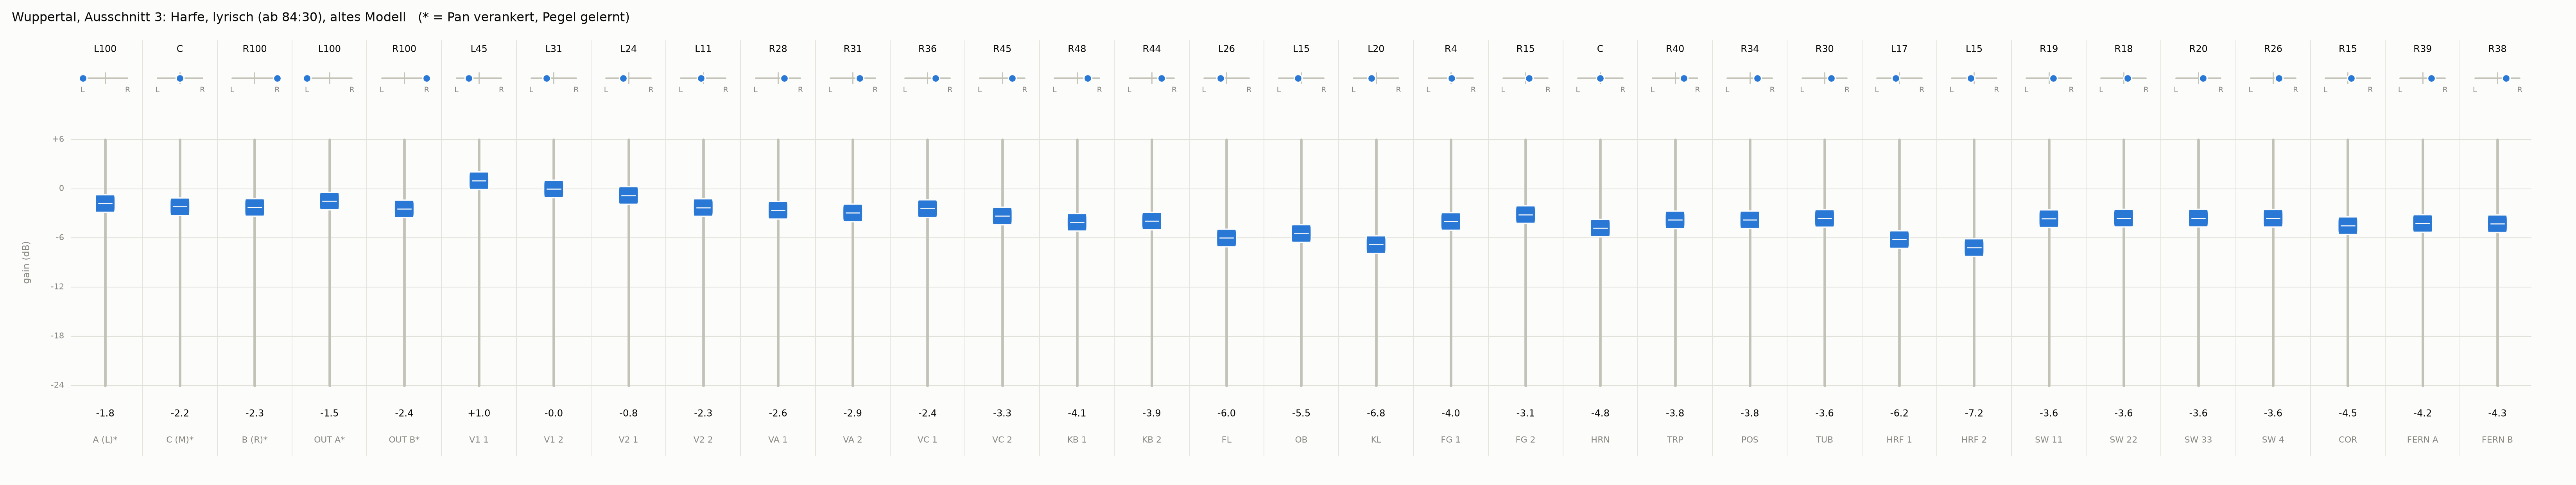
\includegraphics[width=\linewidth]{wuppertal/best_model_3_harfe_lyrisch.png}
\caption{Eigene Konzertaufnahme, lyrischer Ausschnitt mit 33 Spuren. Die
Streicher stehen in der richtigen Reihenfolge von links nach rechts; die
Pegel liegen dagegen eng beieinander. Mit * markierte Spuren sind Anker.}
\label{fig:wuppertal}
\end{figure}

%=====================================================================
\section{Eignen sich eigene Aufnahmen als zusätzliches Trainingsmaterial?}
\label{sec:eigene}

Das Modell soll weiterhin allein aus fertigen Mischungen lernen. Damit hängt
alles an einer Frage: Gibt es zu einer eigenen Aufnahme ein \emph{Ziel}, das
ein statischer Gain/Pan-Mix überhaupt erreichen kann? Die Wuppertaler
Konzertaufnahme eignet sich als Testfall, denn sie enthält eine Spur
\texttt{SUMME} -- die Stereomischung des Tonmeisters über die volle Länge.

\paragraph{Zeitversatz.} SUMME läuft den Einzelspuren um konstant
\SI{12.1}{ms} hinterher (Kreuzkorrelation mit den Hauptmikrofonen). Ohne
Ausgleich ist jede Rückrechnung wertlos ($R^2<0{,}05$); mit Ausgleich lässt
sich die Mischung gut als statische Summe erklären
($R^2 = 0{,}97$ im Solo-Ausschnitt, $0{,}80$ im Tutti). Die zurückgerechneten
Werte bestätigen unabhängig die Aufstellung des Hauptsystems und zeigen, was
der Tonmeister getan hat: Hauptsystem und Außenmikrofone bei
\SIrange{-7}{-11}{dB} tragen die Mischung, die Gesangsstützen liegen
\SIrange{12}{14}{dB} darunter, alle Instrumentenstützen unter \SI{-27}{dB}.

\paragraph{Wie gut ist ein Ziel erreichbar?} Für jedes Kandidaten-Ziel haben
wir Gain und Pan direkt auf das Ziel optimiert -- das ist die Grenze, die kein
Modell unterbieten kann (Abbildung~\ref{fig:feasibility}).

\begin{figure}[h]
\centering
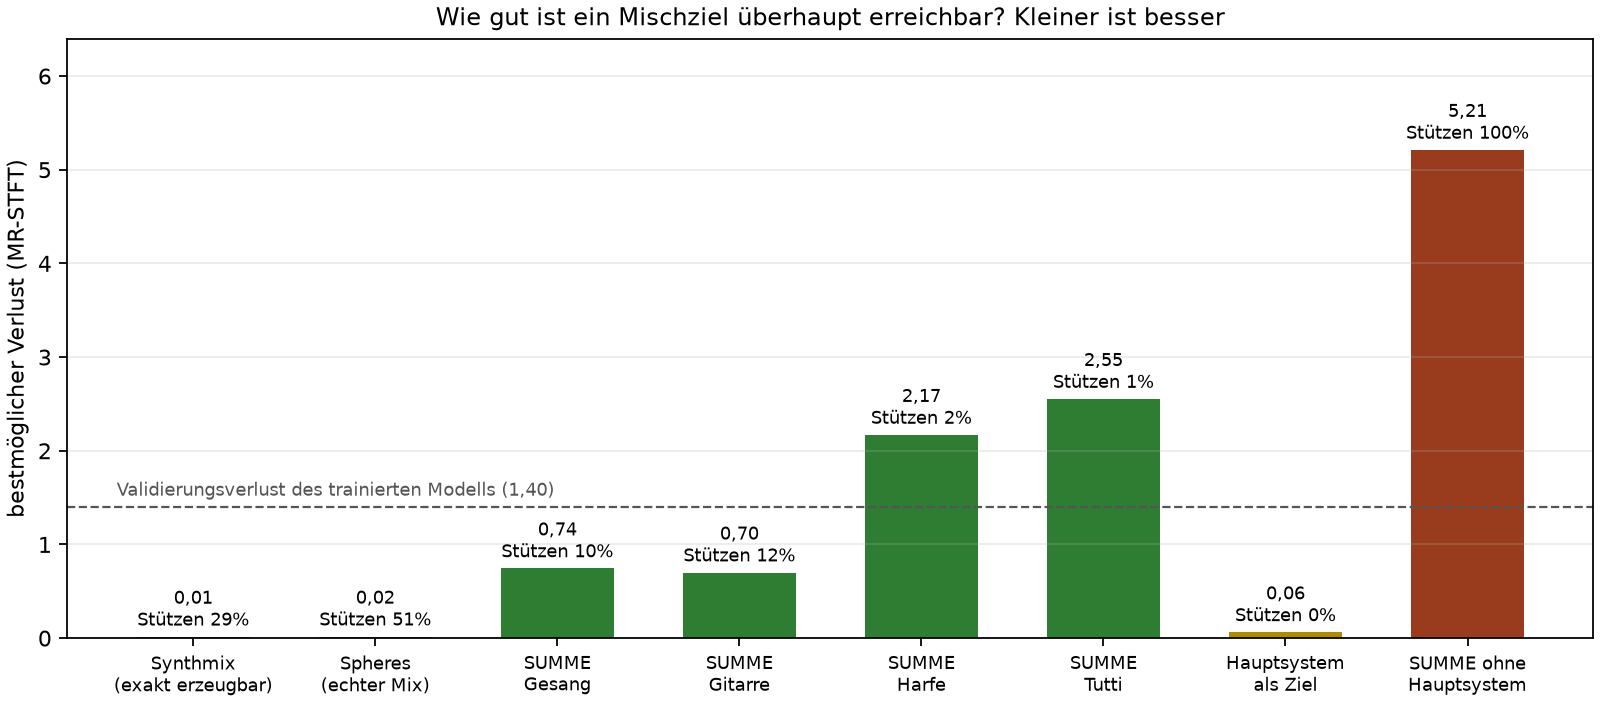
\includegraphics[width=\linewidth]{target_feasibility.png}
\caption{Bestmöglicher Verlust je Ziel, gemessen in der Trainings-Verlust\-funktion.
„Stützen“ ist der Energieanteil der Stützmikrofone in der optimalen Mischung:
Er sagt, wie viel über sie überhaupt zu lernen wäre.}
\label{fig:feasibility}
\end{figure}

\begin{itemize}[nosep]
  \item \textbf{Das Hauptsystem als Ziel ist sinnlos.} Die verankerten
    Hauptmikrofone geben es exakt wieder, die optimale Lösung dreht alle
    Stützen auf null (Energieanteil 0\,\%). Genau in diese Falle führt auch
    das Tree-Ziel von rohem SynthSOD.
  \item \textbf{Ohne Hauptsystem im Eingang ist das Ziel unerreichbar}
    (Verlust 5{,}21). Stützmikrofone allein können das Stereobild eines
    gespreizten Hauptsystems nicht erzeugen -- der Grund, warum es Anker gibt.
  \item \textbf{SUMME ist ein echtes Ziel.} In den beiden Ausschnitten mit
    gestützten Solisten liegt die Grenze bei 0{,}70 bzw.\ 0{,}74, deutlich
    unter dem heutigen Validierungsverlust von 1{,}40, und die Stützen tragen
    \SIrange{10}{12}{\percent} der Energie.
  \item \textbf{Aber nur in Teilen des Konzerts.} In Harfen- und
    Tutti-Ausschnitt steigt die Grenze auf 2{,}2 bis 2{,}6 und der Anteil der
    Stützen fällt auf \SIrange{1}{2}{\percent}. Dort dominieren Reglerfahrten,
    Hall und Klangbearbeitung -- alles, was ein statisches Modell nicht
    abbilden kann. Training auf solchen Ausschnitten hieße, Rauschen zu lernen.
\end{itemize}

\subsection{Das Konzert im Training: Der Verlust täuscht}
\label{sec:konzertlauf}

Wir haben es ausprobiert. Aus dem Konzert wurden \num{124} Fenster von
\SI{30}{s} geprüft; \num{11} waren zu leise (Applaus, Pausen), \num{80} lagen
unter der Güteschwelle, \num{33} blieben übrig -- \SI{16.5}{min} Material mit
$R^2$ zwischen $0{,}95$ und $1{,}00$, alle aus den ersten 63 Konzertminuten.
Diese kamen zu den 68 bisherigen Stücken dazu, sonst wurde nichts geändert.
Ein zusammenhängender Block von Minute 44 bis 63 wurde zurückgehalten;
benachbarte Fenster klingen fast gleich, eine zufällige Aufteilung würde
Trainingsmaterial in die Bewertung durchsickern lassen.

\begin{table}[h]
\centering\small
\begin{tabular}{@{}llrr@{}}
\toprule
Zurückgehalten von & Maß & bisheriges Modell & Konzert-Modell \\
\midrule
beiden Läufen & Pan-Fehler (Streichquartett) & \textbf{\SI{4.20}{\degree}} & \SI{6.53}{\degree} \\
beiden Läufen & Verlust (Streichquartett) & \textbf{1,26} & 2,68 \\
beiden Läufen & Verlust (9 Konzertfenster) & 18,91 & \textbf{3,27} \\
beiden Läufen & Pan-Fehler (Konzert; Mitte \SI{28.6}{\degree}) & \SI{29.20}{\degree} & \SI{28.65}{\degree} \\
beiden Läufen & Gain-Fehler (Konzert; konstant \SI{8.70}{dB}) & \SI{8.62}{dB} & \SI{9.46}{dB} \\
nur neuem Lauf & Gain-Fehler (echte Mischung; konstant \SI{4.92}{dB}) & -- & \SI{6.29}{dB} \\
\bottomrule
\end{tabular}
\caption{Gruppenweise gemessen, weil der Validierungsverlust der beiden Läufe
nicht vergleichbar ist: Der Bewertungssatz hat sich durch die neuen Fenster
verändert.}
\end{table}

Auf Konzertmaterial fällt der Verlust um das Sechsfache -- und trotzdem hat das
Modell das Mischen nicht gelernt. Seine Positionen treffen den Mitte-Tipp auf
ein halbes Grad genau, seine Pegel sind schlechter als ein einziger konstanter
Wert für alle Spuren. Gelernt hat es das grobe \emph{Pegelregime} einer
Aufnahme mit 33--37 Spuren, also wie weit alles heruntergezogen werden muss.
Das belohnt der Verlust stark, denn es betrifft jede Spur gleichzeitig; das
bisherige Modell kannte höchstens 22 Spuren und lag hier weit daneben.

Gleichzeitig hat der Zugewinn anderswo gekostet: Auf einem Stück, das
\emph{beide} Läufe zurückgehalten haben, stieg der Pan-Fehler von
\SI{4.20}{\degree} auf \SI{6.53}{\degree} und der Verlust verdoppelte sich.

\merke{Ein einzelnes Konzert ist eine Mischphilosophie, ein Saal, eine
Besetzung. \SI{16.5}{min} davon verschieben das Modell in Richtung dieser einen
Aufnahme, statt ihm eine übertragbare Regel beizubringen. Der größte Nutzen der
eigenen Aufnahme liegt deshalb in der \emph{Bewertung}: Sie liefert die erste
zurückgehaltene echte Mischung des Projekts. Und sie zeigt, wie wenig der
Verlustwert allein aussagt.}

%=====================================================================
\section{Grenzen und offene Punkte}
\label{sec:grenzen}

\begin{itemize}
  \item \textbf{Der Pegel ist der Engpass.} Die Synthmix-Gains sind gewürfelt
    und damit grundsätzlich nicht lernbar; echte Pegelentscheidungen enthält
    nur Spheres, und dort unterscheiden sie sich stark zwischen den Stücken
    (bei Mozart stehen die Streicher vorn, bei Tschaikowsky die Holzbläser).
    Das Experiment in Abschnitt~\ref{sec:spheresexp} zeigt, dass mehr Gewicht
    auf diesen Daten nicht genügt: Das Modell bildet die echten Pegel selbst
    dann nicht nach, wenn es auf ihnen trainiert. Ein gemitteltes Embedding
    und ein Verlust auf Betragsspektren sind dafür zu grobe Werkzeuge.
  \item \textbf{Stauchung zur Mitte.} Bei Unsicherheit ist die Mitte der
    sicherste Tipp; das Modell nutzt die Stereobreite nicht voll aus.
  \item \textbf{Abstand zu echten Aufnahmen.} Die synthetischen Spots haben
    kein Übersprechen, echte schon; im Training gab es 4--22 Spuren, in
    Wuppertal 33--37, teils mit zwei Mikrofonen pro Stimmgruppe.
  \item \textbf{Statische Einstellungen.} Keine Pegelautomation, kein EQ, kein
    Hall, keine Laufzeitkorrektur zwischen Spot und Hauptsystem.
  \item \textbf{Wenig echte Referenzen.} Zwei echte Mischungen reichen nicht,
    um stückabhängige Pegelentscheidungen zu lernen. Im Lauf aus
    Abschnitt~\ref{sec:konzertlauf} wurde erstmals eine echte Mischung
    zurückgehalten (Tschaikowsky): Dort liegt der Pan-Fehler bei
    \SI{8.77}{\degree} gegenüber \SI{14.18}{\degree} für den Mitte-Tipp, der
    Gain-Fehler aber bei \SI{6.29}{dB} und damit \emph{schlechter} als ein
    konstanter Pegel (\SI{4.92}{dB}). Positionen überträgt das Modell also auf
    unbekannte echte Mischungen, Pegel nicht.
  \item \textbf{Der Verlustwert ist ein schlechter Ratgeber.} Er verbesserte
    sich auf Konzertmaterial um das Sechsfache, während die Reglerentscheidungen
    auf dem Niveau trivialer Vergleichswerte blieben
    (Abschnitt~\ref{sec:konzertlauf}). Aussagen über die Qualität einer
    Mischung sollten deshalb immer an Grad und Dezibel gemessen werden, nicht
    am Verlust.
\end{itemize}

%=====================================================================
\section{Vorschlag: Vom Dokument zum Paper}

\begin{table}[h]
\centering\small
\begin{tabularx}{\linewidth}{@{}lX@{}}
\toprule
Paper-Abschnitt & Inhalt aus diesem Dokument \\
\midrule
Einleitung & Abschnitt 1: Aufgabe, Hauptsystem vs.\ Spots, Motivation für statische Gain/Pan-Entscheidungen. \\
Verwandte Arbeiten & Differenzierbares Mischpult \cite{steinmetz2021}, VGGish \cite{hershey2017}, MR-STFT-Verlust \cite{yamamoto2020,arik2019}; L/R-Invarianz bei Steinmetz vs.\ feste Orchesteraufstellung. \\
Methode & Abschnitte 3--7 und Abbildung~\ref{fig:pipeline}; Gleichungen \eqref{eq:mix}, \eqref{eq:ctx}, \eqref{eq:loss}. \\
Daten & Abschnitt~\ref{sec:daten}: Spheres, SynthSOD, Synthmix; Sitzplan und dessen Bestätigung durch echte Tonmeister. \\
Experimente & Pan-Kollaps und dessen Behebung (Verlust mit Kanaltermen), 200-Epochen-Lauf, Spheres-Gewichtung (Abschnitt~\ref{sec:spheresexp}), Eignung eigener Aufnahmen (Abschnitt~\ref{sec:eigene}). \\
Ergebnisse & Pan-Fehler mit Baselines und Rauschgrenze; Spheres; Wuppertal als qualitative Fallstudie. \\
Diskussion & Abschnitt~\ref{sec:grenzen}; besonders: Verlust vs.\ tatsächliche Reglerentscheidungen, und warum eine einzelne Aufnahme das Modell verschiebt statt es zu verbessern. \\
\bottomrule
\end{tabularx}
\end{table}

\paragraph{Noch zu ergänzen.} Quellenangaben für den Spheres- und den
SynthSOD-Datensatz. Beide sind hier bewusst nicht zitiert: Die genauen
Veröffentlichungen liegen uns nicht vor, und geratene Literaturangaben wären
schlimmer als eine offene Lücke. Sie gehören in Abschnitt~\ref{sec:daten} und
ins Literaturverzeichnis, bevor das Paper eingereicht wird.

\begin{thebibliography}{9}\small
\bibitem{steinmetz2021} C.~J. Steinmetz, J.~Pons, S.~Pascual, J.~Serrà:
  \emph{Automatic multitrack mixing with a differentiable mixing console of
  neural audio effects.} Proc.\ IEEE ICASSP, 2021.
\bibitem{hershey2017} S.~Hershey et~al.: \emph{CNN architectures for
  large-scale audio classification.} Proc.\ IEEE ICASSP, 2017.
\bibitem{yamamoto2020} R.~Yamamoto, E.~Song, J.-M.~Kim: \emph{Parallel
  WaveGAN: A fast waveform generation model based on generative adversarial
  networks with multi-resolution spectrogram.} Proc.\ IEEE ICASSP, 2020.
\bibitem{arik2019} S.~Ö. Arık, H.~Jun, G.~Diamos: \emph{Fast spectrogram
  inversion using multi-head convolutional neural networks.} IEEE Signal
  Processing Letters 26(1), 2019.
\bibitem{kingma2015} D.~P. Kingma, J.~Ba: \emph{Adam: A method for stochastic
  optimization.} Proc.\ ICLR, 2015.
\end{thebibliography}

\end{document}
